%\documentclass[journal]{vgtc}                % final (journal style)
\documentclass[review,journal]{vgtc}         % review (journal style)
%\documentclass[widereview]{vgtc}             % wide-spaced review
%\documentclass[preprint,journal]{vgtc}       % preprint (journal style)

%% Uncomment one of the lines above depending on where your paper is
%% in the conference process. ``review'' and ``widereview'' are for review
%% submission, ``preprint'' is for pre-publication, and the final version
%% doesn't use a specific qualifier.

%% Please use one of the ``review'' options in combination with the
%% assigned online id (see below) ONLY if your paper uses a double blind
%% review process. Some conferences, like IEEE Vis and InfoVis, have NOT
%% in the past.

%% Please use the ``preprint''  option when producing a preprint version
%% for sharing your article on an open access repository

%% Please note that the use of figures other than the optional teaser is not permitted on the first page
%% of the journal version.  Figures should begin on the second page and be
%% in CMYK or Grey scale format, otherwise, colour shifting may occur
%% during the printing process.  Papers submitted with figures other than the optional teaser on the
%% first page will be refused. Also, the teaser figure should only have the
%% width of the abstract as the template enforces it.

%% These few lines make a distinction between latex and pdflatex calls and they
%% bring in essential packages for graphics and font handling.
%% Note that due to the \DeclareGraphicsExtensions{} call it is no longer necessary
%% to provide the the path and extension of a graphics file:
%% 
\includegraphics{diamondrule} is completely sufficient.
%%
\ifpdf%                                % if we use pdflatex
  \pdfoutput=1\relax                   % create PDFs from pdfLaTeX
  \pdfcompresslevel=9                  % PDF Compression
  \pdfoptionpdfminorversion=7          % create PDF 1.7
  \ExecuteOptions{pdftex}
  \usepackage{graphicx}                % allow us to embed graphics files
  \DeclareGraphicsExtensions{.pdf,.png,.jpg,.jpeg} % for pdflatex we expect .pdf, .png, or .jpg files
\else%                                 % else we use pure latex
  \ExecuteOptions{dvips}
  \usepackage{graphicx}                % allow us to embed graphics files
  \DeclareGraphicsExtensions{.eps}     % for pure latex we expect eps files
\fi%

%% it is recommended to use ``\autoref{sec:bla}'' instead of ``Fig.~\ref{sec:bla}''
\graphicspath{{figures/}{pictures/}{images/}{./}} % where to search for the images


\usepackage{microtype}                 % use micro-typography (slightly more compact, better to read)
\PassOptionsToPackage{warn}{textcomp}  % to address font issues with \textrightarrow
\usepackage{textcomp}                  % use better special symbols
\usepackage{listings}
\usepackage{listingsutf8}
\usepackage{mathptmx}                  % use matching math font
\usepackage{times}                     % we use Times as the main font
\renewcommand*\ttdefault{txtt}         % a nicer typewriter font
\usepackage{cite}                      % needed to automatically sort the references
\usepackage{color}
\usepackage{xcolor}
\usepackage{tabu}                      % only used for the table example
\usepackage{booktabs}                  % only used for the table example

\usepackage{algorithm}
\usepackage{algorithmicx}
\usepackage{algpseudocode}
\usepackage{amsmath}
\usepackage{comment}
\usepackage{float}
\usepackage{multirow}
\usepackage{caption}
\usepackage{stfloats}
%\usepackage{ulem}
%\usepackage{fontspec}
%\usepackage{geometry}

\def\degree{${}^{\circ}$}

%%%%%%%%%%%%%%%%%%%%%%%%%%%%%%%%%%%%%%%%%%%%%%%%%%%%%%%%%%%%%%%%%%%%
% First revision
\newcommand{\mm}[1]{\textcolor{red}{#1}}
%\newcommand\reduline{\bgroup\markoverwith{\textcolor{red}{\rule[0.5ex]{2pt}{0.4pt}}}\ULon}
%\newcommand{\removed}[1]{\reduline{#1}}
\newcommand{\rmrm}[1]{\sout{#1}}

\def \firstclean{} % remove this comment to generate a clean version
\ifx\firstclean\undefined
\usepackage{ulem}
\else
 % \renewcommand{\remark}[1]{\iffalse #1 \fi}
 \renewcommand{\rmrm}[1]{\iffalse #1 \fi}
 \renewcommand{\mm}{}
\fi


\onlineid{1021}

%% declare the category of your paper, only shown in review mode
\vgtccategory{Research}
%% please declare the paper type of your paper to help reviewers, only shown in review mode
%% choices:
%% * algorithm/technique
%% * application/design study
%% * evaluation
%% * system
%% * theory/model
\vgtcpapertype{Technique}

%% Paper title.
\title{ARLayout: Massive Physical Targets Visual Re-Layout in Mobile Augmented Reality}
% MomentRecapturer: Target Visual Re-grouping, Reranking and Relayout by Augmented Reality

% Re-grouping, Re-ranking and Re-layout
 
%% This is how authors are specified in the journal style

%% indicate IEEE Member or Student Member in form indicated below
\author{Roy G. Biv, Ed Grimley, \textit{Member, IEEE}, and Martha Stewart}
\authorfooter{
%% insert punctuation at end of each item
\item
 Roy G. Biv is with Starbucks Research. E-mail: roy.g.biv@aol.com.
\item
 Ed Grimley is with Grimley Widgets, Inc.. E-mail: ed.grimley@aol.com.
\item
 Martha Stewart is with Martha Stewart Enterprises at Microsoft
 Research. E-mail: martha.stewart@marthastewart.com.
}

%other entries to be set up for journal
\shortauthortitle{Biv \MakeLowercase{\textit{et al.}}: Global Illumination for Fun and Profit}
%\shortauthortitle{Firstauthor \MakeLowercase{\textit{et al.}}: Paper Title}

%% Abstract section.
\abstract{
The increasing popularity of VR/AR/MR devices has
attracted a great deal of attention from researchers in the communities of
virtual reality, visualization and human-computer interaction.
However, enabling the public to create AR-based visualizations
is challenging due to the steep learning curve of programming on AR devices.
In this paper, we propose \textit{ARLayout}, an authoring tool designed
for non-experts to build AR-based visual re-layouts towards massive physical targets,
such as books, coffees, drinking, foods, eyeshadows or even some toys,
which are captured from the reality world in real-time by the camera of
mobile devices such as mobile phones or tablets.
All the candidate targets can be segmented and labeled by
a convolutional neural network named BOWDA-Net~\cite{Zhu2020},
which just requires a small scale of labeled training 
samples (less than 100 for each case in our experiments).
The textual information is recognized by an OCR algorithm.
The visual re-layouts of the physical targets include highlighting
the search results by fisheye deformation, re-grouping and re-ranking.
Specifically, (1) the fuzzy keywords are input by voice to 
narrow down the number of candidate targets by searching,
while the search results will be highlighted in the AR environment 
to guide them where to find the targets in the reality world.
%, e.g., searching books with fuzzy keywords from massive books in a library.
(2) candidate targets can be re-grouped in the AR environment according to one/multiple of 
their nominal, ordinal or quantitative attributes.
(3) candidate targets can be re-ranked in the AR environment according to one of
their ordinal or quantitative attributes.
We demonstrate the usability, expressiveness and effectiveness 
of \textit{ARLayout} by user study and case study with three usage scenarios in the evaluation.
} % end of abstract

%% Keywords that describe your work. Will show as 'Index Terms' in journal
%% please capitalize first letter and insert punctuation after last keyword
\keywords{Augmented reality, authoring tool, visual layout, physical visualization}

%% ACM Computing Classification System (CCS).
%% See <http://www.acm.org/class/1998/> for details.
%% The ``\CCScat'' command takes four arguments.

\CCScatlist{ % not used in journal version
 \CCScat{K.6.1}{Management of Computing and Information Systems}%
{Project and People Management}{Life Cycle};
 \CCScat{K.7.m}{The Computing Profession}{Miscellaneous}{Ethics}
}

%% A teaser figure can be included as follows
%\teaser{
%  \centering
%  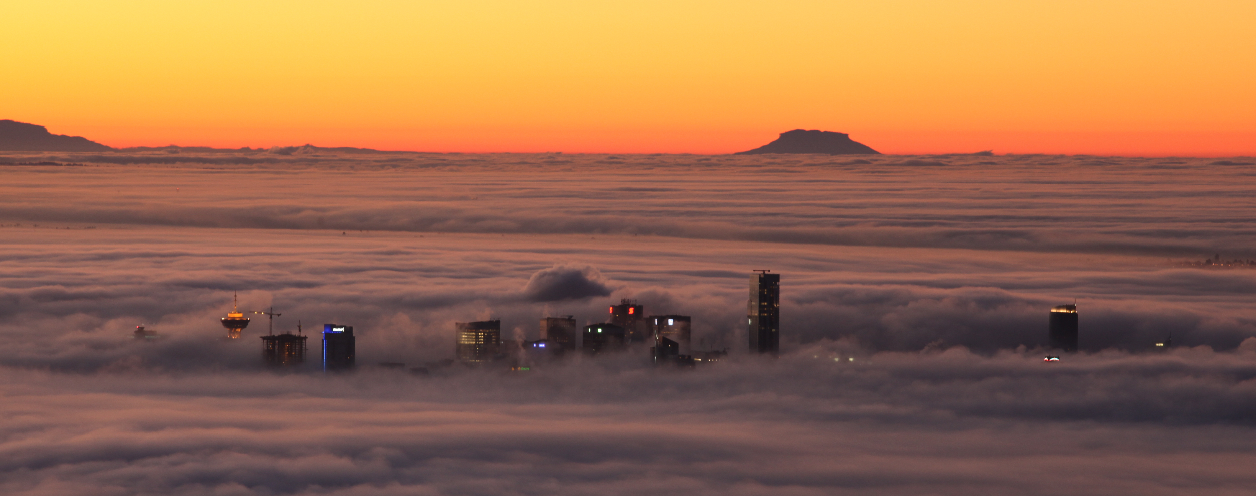
\includegraphics[width=\linewidth]{CypressView}
%  \caption{In the Clouds: Vancouver from Cypress Mountain. Note that the teaser may not be wider than the abstract block.}
%  \label{fig:teaser}
%}

%% Uncomment below to disable the manuscript note
%\renewcommand{\manuscriptnotetxt}{}

%% Copyright space is enabled by default as required by guidelines.
%% It is disabled by the 'review' option or via the following command:
% \nocopyrightspace


\vgtcinsertpkg

%%%%%%%%%%%%%%%%%%%%%%%%%%%%%%%%%%%%%%%%%%%%%%%%%%%%%%%%%%%%%%%%
%%%%%%%%%%%%%%%%%%%%%% START OF THE PAPER %%%%%%%%%%%%%%%%%%%%%%
%%%%%%%%%%%%%%%%%%%%%%%%%%%%%%%%%%%%%%%%%%%%%%%%%%%%%%%%%%%%%%%%%

\begin{document}

%% The ``\maketitle'' command must be the first command after the
%% ``\begin{document}'' command. It prepares and prints the title block.

%% the only exception to this rule is the \firstsection command
%\firstsection{Introduction}

%\maketitle



%%%--------------------------------------------------------------------------------%%%
\firstsection{Introduction}
\label{sec:introduction}

\maketitle


%沉浸式设备的普遍、技术背景、及其优点

The development and the popularity of augmented reality (AR) devices
and the techniques have led to an increasing number of studies
designing new authoring tools or personal visualizations (PV).
PV is designed to help the public get better insight into the data
in a personal context.
Unlike the traditional visualizations that are oriented to domain experts,
PV is less domain-specific and highly focus on
daily life~\cite{Huang2014,Reipschlager2021}.
Chen et al.~\cite{Chen2020} have summarized that
mobile AR techniques have great potential to facilitate PV.

In our everyday life, it is probable that it would take us
a large amount time to find or choose a target object,
e.g., a book, a coffee, a kind of drinking, a cup, a kind of fruit or even an eyeshadow
from massive candidates according to some fuzzy information.
Similarly, it also would take us too much time to filter, group or sort them
by one or multiple additional attributes for better comparison.
The used additional attributes can be summarized into the nominal, the ordinal or the quantitative.

For example, finding a book according to the book name with fuzzy keywords or fuzzy author names
in a library/bookstore (searching/filtering),
and then highlight the search results.
Besides, they would browse all the books and filter them
to get a smaller number of candidate books (e.g., ``Algorithms'', nominal) for further comparisons.
There are two subsequent actions the users would probably take:
(1) Re-grouping. Re-group them according to the publishers (``IEEE'' or ``Springer'', nominal),
book series, topics (e.g., ``dynamic programming'', nominal), or even more additional attributes
instead of the unified classification numbers frequently-used in libraries.
(2) Re-ranking. sort them according to their ratings (ordinal), prices (quantitative)
or even more additional attributes.
The illustrations of the library usage scenarios are shown in~\autoref{fig:intro_relayout_task}.

\begin{figure*}[htb]
%\setlength{\abovecaptionskip}{0.05cm}
%\setlength{\belowcaptionskip}{-0.4cm}
    \centering
    \includegraphics[width=\linewidth]{images/intro_relayout_task.eps}
    \caption{
      The task illustrations on searching (a), re-grouping (b), and re-ranking (c) in AR environment.
      We take the library/bookstore scenario as an example.
    }
    \label{fig:intro_relayout_task}
\end{figure*}

Except for the example of finding/comparing targets from massive candidates, such as the above-mentioned
finding/re-grouping/re-ranking books in a library or a bookstore,
we also note that many people either are hard to distinguish the names of some massive goods like foods or drinking,
or are ambiguous to choose a specific goods from the massive candidates because they
could not tell or remember the major differences of them.
For example, we find that many people are hard to identify different coffees
according to a pre-study investigation of the user study in Section~\ref{sec:evaluation},
such as Caffe Misto, Blonde Roast, Caffe Mocha, Cappuccino, Caffee Americano, Flat White, Pistachio Latte,
Caramel Macchiato, Nitro Cold Brew, Iced Coffee, Irish Cream Cold Brew, White Chocolate Mocha, Iced Pistachio Latte,
or even the combinations of coffees with tea and coffees with milk, etc.
We also find it difficult for them to choose a coffee in a coffee shop
because they cannot remember the major differences of their ingredients (quantitative)
e.g., the total caffeine, calorie, protein, fat, milk, etc,
the price (quantitative) and rating (ordinal)
Is it sweet or sugarless and what the total sugar content (quantitative) or
the place of origin (nominal) is.
For the users who can identify the coffee names but often are ambiguous to
choose a coffee in a coffee shop,
he would further filter the coffee to get a small number of target candidates,
e.g., ``espresso'' or ``white americano'' (searching/filtering),
and then re-group them according to the above-mentioned
nominal, ordinal or quantitative attributes (re-grouping),
or sort them according to the ordinal or quantitative attributes (re-ranking).

We summarize many of such usage scenarios (book, coffee, drinking, fruit, eyeshadow, etc.)
towards \textbf{massive target objects}
in our daily life into three categories according to the tasks and data attributes as follows.
We call them \textbf{visual re-layout for massive targets} in this paper because almost all of them
need to break the original physical layouts in the reality.

\begin{itemize}
\item \textbf{Searching or filtering}: highlight the searched results to provide visual cues
about their physical positions (used attributes: \textbf{nominal (including hue), ordinal}).
\item \textbf{Re-grouping}: re-group the target objects according to one/multiple attributes via breaking the original physical
layouts in AR environment (used attributes: \textbf{nominal (including hue), ordinal, quantitative}).
\item \textbf{Re-ranking}: sort the target objects according to one/multiple attributes via changing the original physical
layouts in AR environment (used attributes: \textbf{ordinal, quantitative}).
\end{itemize}


The above-mentioned visual re-layout for massive targets can be achieved by AR-based authoring PVs.
However, enabling the public especially for the users
with little knowledge about programming
to create AR-based authoring tools is challenging
due to the steep learning curve of programming on AR devices
and the inconvenient offline workflow where users should
work back-and-forth between AR devices and desktop PCs~\cite{Chen2020}.


In this paper, we propose \textit{ARLayout}, an authoring PV tool designed
for non-experts to build AR-based visual re-layouts based on real-time videos
towards massive physical targets,
which are captured from the camera of personal mobile devices such as mobile phones or tablets.
All the candidate targets can be segmented and labeled by
a convolutional neural network named PaddleSeg~\cite{Liu2019,Liu2021a},
which just requires a small scale of labeled training samples (less than 100 in our three cases).
The textual information about the targets is recognized by an OCR algorithm.
The visual re-layouts can be achieved by above-mentioned
searching (or filtering), re-grouping and re-ranking, etc.
First, searching is used to narrow down the number of candidate targets
where the search keywords are input by voice.
The search results will be highlighted in the AR environment to guide them where to find
the target in the reality world.
%, e.g., searching books with fuzzy keywords from massive books in a library.
Secondly, candidate targets can be re-grouped in the AR environment according to one or even multiple of their
nominal, ordinal or quantitative attributes.
Thirdly, candidate targets can be re-ranked in the AR environment according to one of
their ordinal or quantitative attributes.
In the experiments, we evaluate the proposed \textit{ARLayout} by
user study and three usage scenarios,
which demonstrate the usability, effectiveness and expressiveness of the tool.



%底下这一段直接放在discussion而不是放到
%Therefore, the PV tasks of this paper are also different from them due to the larger data scale.
%We focus on searching/filtering, re-grouping and re-ranking according to
%the additional attributes of massive physical targets
%through the visual re-layouts of them,
%instead of augmenting the existing static visualizations in PapARVis~\cite{Chen2020a}.
%Besides, the visual presentation is different.
%We focus on AR-based fisheye highlighting, virtual word cloud and virtual small multiples for better comparisons
%for massive targets instead of virtual glyphs in MARVisT~\cite{Chen2020}.



%三个CASE的例子可以在这里分别讨论一下场景,尤其是前面两个例子,
%找书,但是图书馆或书店是分别按照分类号或者畅销程度进行排列,况且,有些书并没有正确按照分类号排列,
%所以我们做了pre study,发现几乎所有测试者都表示曾经在图书馆或者书店里找一本书要找很久,
%此时,用户在借阅或购买之前可能要对目标书籍进行多个维度的分组对比等等,
%或者对价格,评价进行排序
%
%咖啡也是,几乎被测试者不知道各种咖啡的成份含量,也不知道不同各类成分的最大不同之处,不知道
%能量,含糖量,是否包括牛奶等。
%
%眼影的也可以说下。




%与这个工作MARVisT一定要详细讨论不同点,我们针对的是大量杂乱无章的对象,
%所以给图像识别,重布局会带来很大的挑战
%做的方面不一样这个是其次,最重要的是就是我刚说的这个,我们针对的是大量杂乱无章的对象,
%所以给图像识别,重布局会带来很大的挑战
%数据量更大,数据空间更大,带来了新的问题,带来了新的挑战,所以也带来了新的方法












\section{Related Work}
\subsection{AR Visualizations}

Embedded data representations links visualization systems to physical things~\cite{Willett2017}.
Augmented Reality (AR), as an important method to combine digital data and physical world,
can visualize data in the physical space to facilitate certain visual explorations and integrate visualization into personal ideas and preferences~\cite{Butscher2018}.
When displaying ubiquitous data integrated into the everyday life,
spatial immersion issues like depth perception, data localization and object relations become relevant.
Works related to AR nowadays can be roughly classified as mobile (or tablets) hand-based systems~\cite{ElSayed2015},
and head-mounted displays (HMD) systems~\cite{Herr2017} according to the computing paradigm.
The Hololens device includes a depth sensing camera that estimates the
distance of each pixel in view and stitches together a mesh
or spatial map
of the environment~\cite{Evans2017}.
Similar technologies are also available in Google Tango~\cite{MarderEppstein2016} and Intel Realsense~\cite{Keselman2017}.
The software development kit (SDK)~\cite{Amin2015} provides ordinary programmers
with more freedom and flexibility
to use their own inspiration to design excellent AR applications,
such as ARToolkit~\cite{Wagner2003, Hirokazu2002},
Vuforia~\cite{Cushnan2013},
ARCore for Android~\cite{ArCore},
and Mixed for Microsoft Universal Windows platform (UWP) Reality Toolkit~\cite{Liberty2018}.
A-Frame~\cite{aframe} which enables create immerse visualization scenes in the browser integrating by WebVR~\cite{webvr} content within HTML.

An inevitable direction of AR development is simultaneous localization and mapping
(SLAM)~\cite{Davison2003} technology, which can build a model simulating the real environment through the background process based on panoramic 3-D reconstruction.
Motion tracking based on MonoSLAM~\cite{Davison2007} has problems such as extensive calculation,
long work time, existing scale ambiguity~\cite{Davison2007}, and difficulty detecting feature points when the device is moving fast.
The integration of inertial measurement unit IMU~\cite{Jones2011} to get six degrees of freedom (6DOF)~\cite{Leutenegger2015} of the device
plays a complementary role in improving its refresh rate and accuracy.

AR visualization has been applied to many fields.
In outdoor visualization,
the CityViewAR~\cite{Lee2012} provides information about destroyed buildings and historical sites that are affected by the earthquakes.
Then,
AR in the interpretation of terrain relief~\cite{Carrera2018} shows a great usability,
which serves as a motivational tool for the 3-D visualization.
Applications in the newly emerging field of Augmented Reality Art
show the paradigmatic potential of AR as a new artistic medium~\cite{Geroimenko2012} .

\subsection{Personal Visualization}
Personal Visualization fits personal routines, situating visualization in a real-world context, and arousing users' interests.
Visualization (Vis) and visual analytics (VA) offer substantial opportunities to help individuals gain insights about themselves.
The combination of large interactive displays with personal head-mounted Augmented Reality (AR)~\cite{Reipschlager2021} for information visualization to facilitate data exploration and analysis.
Personal Visualization and Personal Visual Analytics (PV \& PVA) are defined in terms of personal context~\cite{Huang2014}.
It broadens the scope of visualization and visual analytics,
including casual InfoVis~\cite{Pousman2007}, InfoVis for the Masses~\cite{Danziger2008},
persuasive computing~\cite{Fogg1998} and personal informatics (PI)~\cite{Li2010, Li2010a}.
Researchers have presented mobile PV systems~\cite{Chiu2009, Kim2010, Kjeldskov2012}
to visualize daily information collected from peripheral sensors.
Besides, in physical PV systems express abstract data in a physical form~\cite{Jansen2015}.
Jansen et al.~\cite{Jansen2013, Jansen2015a} shows physical visualization can improve the users' efficiency in retrieval tasks.

Some researchers have designed physical visualization to visualize personal data.
Khot et al.~\cite{Khot2014} transforms heart rate data into five kinds of 3-D printed material artifacts,
and Stusak et al.~\cite{Stusak2014}designs four types of sculptures to visualize running activities and
evaluates their usability through a field study.
Huang et al.~\cite{Huang2016} designs a behaviour feedback visualization tool
to help people improve their health or personal well-being or to carry out sound environmental sustainability practices.
Moreover, understanding and reasoning about personal data is of great importance,
e.g., pedometer counts~\cite{Stusak2014}, blood pressure readings~\cite{Goh2016} or home electricity consumption~\cite{Monigatti2010},
It can be chanllenging while gaining a deeper understanding of one's current practices and learning how to make a change when using data alone.

\subsection{Visualization Authoring Tools}
The field of immersive visualization makes use of Augmented Reality techniques to successfully support users in visualizing data.
However,
designing visualizations in immersive environments can be intricate,
which needs consideration of issues such as shadows~\cite{Allen1999, Mamassian1998, Yonas1978}, occlusion, and additional argumentations.
Nowadays several techniques are available that allow real-time rendering of shadows in augmented reality scenes~\cite{Tsuda2006, Wither2005}.
Different approaches are used to modify the appearance of occluding objects to uncover the hidden ones.
Cut-aways can be found for instance~\cite{Bichlmeier2007, Furmanski2002},
and transparencies in combination with masks are used~\cite{Mendez2009}.

On one hand,
researches have proposed several toolkits that allows interactive authoring and exploration of data visualisation in immersive environments.
With MARVisT~\cite{Chen2020}, users without visualization expertise can bind data to real-world objects to create expressive AR glyph-based visualizations rapidly and effortlessly.
DXR~\cite{Sicat2019} further provides a GUI for easy and quick edits and previews of visualization designs in-situ, i.e., while immersed in the virtual world.
IATK~\cite{Cordeil2019} allows for easy assembly of visualisations through a grammar of graphics that a user can configure in a GUI--in addition to a dedicated visualisation API.
PapARVis~\cite{Chen2020a} designs an environment that can debug both static and virtual content simultaneously.
Automated Window/Icon/Menu/Pointing Device User Interface (WIMP-UI)~\cite{WIMPUI} generation has been considered a promising technology for at least two decades.
iVisDesigner~\cite{Ren2014} achieves high interactive expressiveness through conceptual modularity, covering a broad information visualization design space.
A mixed-initiative system Voyager that supports faceted browsing of recommended charts chosen according to statistical and perceptual measures~\cite{Wongsuphasawat2016}.

On the other hand,
an API known as OpenGL bridges the gap between piles of raw data and extremely complicated three-dimensional animation in a way~\cite{Shreiner2013}.
The graphical demands of some of the applications have impeded their successful settlement in Web scenarios,
thus people begin to use WebGL~\cite{Parisi2012} to articulates a large portion of the rendering task in the client machine.
Declarative visual design language can customizes built-in chart types, such as Echarts~\cite{Li2018} and D3~\cite{Zhu2013}.
A high-level grammar Vega-lite~\cite{Satyanarayan2017} provides visual encoding rules and a composition algebra that enables rapid specification of interactive data visualizations.
Some features are used to analyze, display and manage the 3-D structure of the molecules by Vega~\cite{Pedretti2002}.

\begin{table}[htp]
%\setlength{\abovecaptionskip}{0.05cm}
%\setlength{\belowcaptionskip}{-0.4cm}
    \centering
    \includegraphics[width=\linewidth]{images/discussion_relatedwork_cmp.eps}
    \caption{
        Comparison to the most related recent work about authoring PV tools towards AR or VR visualizations.
        The most related approaches include:
        DXR~\cite{Sicat2019}, Augmented Virtual Teleportation (AVT)~\cite{Rhee2020}, 
        Situated Analytics (SA Vis)~\cite{ElSayed2015}, Data Visceralization (VR Visc)~\cite{Lee2021a},
        Shared Surfaces and Spaces (VR Collab Vis)~\cite{Lee2021}, PapARVis~\cite{Chen2020a},
        MARVisT~\cite{Chen2020}.
        The workflow can be categorized into PV (single user in a personal context),
        single user or collaborative users.
    }
    \label{tab:discussion_relatedwork_cmp}
\end{table}



\subsection{Relationship with The Most Related Work}
\label{sec:relatedworkcomparison}

We note that there are some most related AR-based tools on authoring visualizations~\cite{Chen2020,Chen2020a}, etc.
We summarize and discuss the differences between \textit{ARLayout} and the most related ones
as shown in Table~\ref{tab:discussion_relatedwork_cmp}
according to the data scale, tasks (augmented information, searching, re-grouping, re-ranking),
visual presentations (glyph, small multiples, fish eye highlight), workflow (personal, single or collaborative).

First, the biggest differences between our work and the existing AR-based PV tools like MARVisT~\cite{Chen2020}
are the data scale and the tasks, we focus on massive targets especially for
the number is larger than 40 or even thousands of targets like books in a library/bookstore
while most of AR-based PV tools just focus on physical targets with the number
smaller than $30$~\cite{Chen2020}, PapARVis~\cite{Chen2020a} ($\leq 5$) and Situated Analytics~\cite{ElSayed2015} ($\leq 5$).
The large data scale of this paper poses a new challenge in image segmentation, object labelling, textual information
recognition and the AR-based data presentation.

Second, we focus on searching/filtering, re-grouping and re-ranking according to
the additional attributes of massive physical targets
through the visual re-layouts of them,
instead of augmenting the existing static visualizations in PapARVis~\cite{Chen2020a}.
The PV tasks are different from the most related work due to the larger data scale of \textit{ARLayout}.
On the one hand, our work can process more than a thousand candidate targets at the same time,
allowing users to access most of the information in the scenario.
On the other hand, this feature on data scale also makes our work adaptive to more scenarios,
rather than limited to some specific scenarios with only a few targets.

Third, the visual presentations of \textit{ARLayout} are different.
We focus on AR-based fisheye highlighting, virtual word cloud and virtual small multiples for better comparisons
for massive targets instead of virtual glyphs~\cite{Chen2020}.

Fourth, there are a series of methods focus on the virtual targets in the virtual space or virtual screen,
which are more close to virtual reality (VR)~\cite{Sicat2019,Rhee2020,Lee2021} instead of AR.

%The most related work of \textit{ARLayout} are some authoring tools
%towards AR or VR visualizations~\cite{Sicat2019, Rhee2020, ElSayed2015, Lee2021a, Lee2021, Chen2020a, Chen2020}.
% As shown in Table~\ref{tab:discussion_relatedwork_cmp},
% we compare them from ten aspects:
% target number, virtual space, augmented information,
% searching, re-grouping (multi-attris), re-ranking (multi-attris),
% glyph vis, small multiples, fish eye highlight, single or collaborated.
% We summarize them into four criterias:
% data scale, task,
% visual presentation, workflow.


%~\cite{Sicat2019, Rhee2020, ElSayed2015, Lee2021a, Lee2021, Chen2020a, Chen2020}
%DXR:Sicat2019
%PapARVis:Chen2020a
%MarVisT:Chen2020
%AR Info Vis:Reipschlager2021
%VR Collab:Lee2021
%AVT:Rhee2020
%SA Vis:ElSayed2015



\section{Design Rationale}
\label{sec:design}
We illustrate the design goal, design considerations and design details of \textit{ARLayout} in this section.
% This part mainly discusses the design rationale of \textit{ARLayout},
% including the considerations and the details of \textit{ARLayout}.

\subsection{Design Goals}
% Based on the characteristics of ARLayout,
% combined with user’s interaction experience,

The target users of \textit{ARLayout} are the people who are not the experts in a given domain.
The ``users'' or ``target users'' in this paper refer to this group of users,
if they are not specially specified.

We summarize the following four design goals of \textit{ARLayout} according
to the requirements collected from the daily life of the target users:
% These design considerations will be refined over time under the guidance of an iterative strategy.

\begin{itemize}
\item G1: enable the target users to search/filter massive physical targets,
and then highlight the results to guide them where they are in reality.
\item G2: enable the users to re-group the physical targets according to their grouping comparison tasks.
\item G3: enable the users to re-rank/sort the physical targets according to their ordinal or quantitative comparison tasks.  %// add & cut in coding space.
\item G4: provide extra augmented information in AR environments according to their tasks.
\end{itemize}



\subsection{Design Considerations and Design Details}

We also summarize the design considerations and design details of \textit{ARLayout}
towards the design goal (G1-G4):

First, the tool should be designed to enable the target users to search/filter the massive physical targets
by one or multiple fuzzy keywords input by voice, because voice input is simple-to-use in the public's PV context,
such as a library, a bookstore, or a coffee shop.
The input method by virtual keyboard should be also provided when it is not convenient to input a voice.
The search results should be \textbf{highlighted by visual cues} to guide the users where they are in reality.
Specifically, we use flashing to highlight the search results and further
provide an AR-based \textbf{fisheye deformation design} to highlight their positions in reality.

Second, the tool should be designed to enable the users to re-group the physical targets
according to their grouping comparison tasks (\textbf{visual re-layouts}),
e.g., re-grouping them according to one/multiple of their nominal, ordinal or quantitative attributes,
because grouping can help users better compare target candidates according to the experience in our daily life.

Third, the tool should be designed to enable the users to re-rank the disordered physical targets,
or re-rank them according to one or multiple additional attributes (\textbf{visual re-layouts}).
For example, books in a library are usually sorted by classification number or index number,
which can not satisfy users' kinds of ranking needs, e.g., sorting them by the rating, price,
publisher or publish year.
Similarly, the books in a bookstore are often sorted by user groups,
more information like ratings and prices are ignored.
As a result, readers may spend a great deal of time finding an ideal book on the bookshelves.

Fourth, in people's daily life, the provided information alongside a target is usually not enough.
For example, we can see the title of a book, the name and the price of a cup of coffee.
However, the rating of a coffee, a book or a food,
and the ingredients or drinks, foods, fruits are often not provided clearly
to make comparisons.
Therefore, the tool should be designed to display extra information which is often hidden from users
or is inconvenient for them to compare.
Actually, this kind of augmented information can be provided by \textbf{juxtaposition}
or using \textbf{small multiples} to help them make a better choice.
Except for the re-layouts, the sorted information such as the price and the rating can be visualized by
\textbf{bar charts} or \textbf{line charts} in AR.

The extra textual information such as the textual ratings
or detailed textual descriptions about the current targets can be visualized
by using \textbf{word cloud} in the style of \textbf{small multiples} to show their keywords,
which are generated from online review.
Besides, it is significant that the re-layout effects
could be integrated into reality without confusion.
In addition, users may be non-experts unfamiliar with programming or AR.
The inaccurate recognition, rough interaction and tedious interface
will add their cognitive burden in a messy situation.
Therefore, \textit{ARLayout} will provide an intuitive interface
with concise interactions to avoid causing visual clutter and discomfort.


\begin{figure}[htp]
%\setlength{\abovecaptionskip}{0.05cm}
%\setlength{\belowcaptionskip}{-0.4cm}
    \centering
    \includegraphics[width=\linewidth]{images/design_overview.eps}
    \caption{
        The structural design of ARLayout,
        including simplified data processing, data transmission, and data presentation process.
    }
    \label{fig:design_overview}
\end{figure}



\subsection{Design Details: System Workflow Design}

As shown in~\autoref{fig:design_overview}, \textit{ARLayout} consists of two parts.
The first part is the mobile client, which is used to take pictures or record a real-time video and then renders objects in AR.
The second part is the server, which is employed to process almost all of the data.
The overall processing are described as follows:
The mobile client constantly takes pictures or record a real-time video of massive targets and sends them to the server.
The remote server processes those pictures or key frames, recognizing target objects in them in real-time,
and sends targets' data back to the mobile client,
which displays them in new layouts.
This workflow design has two considerations:


\textbf{Separation of heavy computing and AR presentation}:
Unlike traditional applications,
\textit{ARLayout} shifts most of the computational intensive tasks to the server.
The mobile client only needs to send the requests in multi-thread to ensure real-time target recognition.
This enables \textit{ARLayout} to handle a large amount of data
% which makes it response faster and more efficiency
without adding a heavy burden to the user’s mobile device or influencing user's interaction experience.
In the library/bookstore scenario, for example, more than \textbf{a thousand} books can be recognized in AR
with panoramic pictures.

\textbf{Separate processing of text and texture}:
The text and texture in one picture usually contains most of our desired information.
We apply different neural network to process these two kinds of data.
% Most information are contained in text or texture
% For the text and texture in the image, are combined into structured data,
% using different neural network processing.
This makes our model not only suitable for situations where information is expressed more in text,
such as library or cafe,
but also for situations where texture contains more information,
such as eyeshadows in cosmetics shops.
For more implementation details, please refer to Section~\ref{sec:implementation}.



% These three methods changes targets' attributes into position information
% to one criterion that's easily perceived by human eyes,
%  that's inefficiently perceived by human eyes to another
% which exploits the capabilities of human's visual system,
% These three methods helps
%as shown in~\autoref{fig:design_relayout}.
% e.g., re-ranking books by their prices encodes books' quantitative information to position infomation,
% enabling the user to easily compare the prices of them.


%\textbf{Searching}.
%\textit{ARLayout} allows the user to achieve
%preseted information of targets automatically in different scenarios.
%Visual feedback will be provided after each search,
%such as magnifying and highlighting the querying results.
%In this way, the targets' nominal and quantitative attributes
%are tranformed to highlight colors and scaled volumes,
%which makes the information easily perceived by the user.
%
%
%\textbf{Re-grouping}.
%\textit{ARLayout} allows the user to arbitrarily group target objects
%according to the preset dimensions in the scenario.
%Different groups are placed separately with group name shown by the side,
%e.g., book groups placed on different layers of the bookshelves, or coffee names in different areas of the menu.
%% For example, the user can choose to re-group books by their publishers,
%% authors or other attributes.
%% \textit{ARLayout} creates new bookshelves and displays different groups on different layers,
%% which encodes books' nominal information (publisher) with position.
%
%\textbf{Re-ranking}.
%\textit{ARLayout} allows the user to sort targets based on information in different dimensions.
%Sorted targets are lined up in certain order in front of the user,
%making the finding and comparing process intuitive and clear.















\section{Evaluations}
\label{sec:evaluation}

\subsection{Case Scenarios}
We choose three typical scenarios where people often experience confusion
when finding or choosing targets in a messy situation:
(1) Find ideal books in the library or book store.
(2) Choose coffees that suits one's taste in a coffee shop
(3) Choose a suitable eyeshadow palette among many palettes in a cosmetics shop.

We discuss the usage of searching, re-grouping, and re-ranking in the three common scenarios,
as well as different dimensions concerning the three information categories mentioned in~\autoref{sec:design},
as shown in~\autoref{fig:design_compare}.
% in order to better illustrate the usage scenarios of searching, re-grouping, and re-ranking,
% we discuss how these processes embed in three common \textit{ARLayout} usage scenarios

% concerning three basic attributes in visualization: nominal, ordinal, and quantitative.

\begin{figure}[htp]
%\setlength{\abovecaptionskip}{0.05cm}
%\setlength{\belowcaptionskip}{-0.4cm}
    \centering
    \includegraphics[width=\linewidth]{images/design_compare.eps}
    \caption{
    Building re-layouts with different methods in three scenarios (library, coffee shop and eyeshadow).
    Targets in different scenarios have different kinds of attributes.
    }
    \label{fig:design_compare}
\end{figure}

In library scenario, the user can search books according to both nominal and quantitative attributes,
e.g., searching for books written by a given author, or for books at a given price;
The user can also re-group books by ordinal or quantitative attributes,
e.g., grouped by rating or by price intervals.
Books can also be re-ranked by ordinal and quantitative attributes
e.g., sorting books in ascending order based on the price.
Besides,
targets in coffee shop and eyeshadow scenarios have less information than the library scenario,
so they doesn’t involve quantitative or ordinal re-grouping.
The eyeshadows cannot be re-ranked as well due to their abstract features.






To verify the usability and effectiveness of \textit{ARLayout},
we design 5 tasks for participants to accomplish:
two in the library, two in a simulated coffee shop, and one in a simulated cosmetics shop.
The 5 tasks represent most of the possible situations happen in these 3 three places,
where people may want to choose a suitable object in a complex scene.
In accord with our 3 goals mentioned above,
the study aimed to evaluate \textit{ARLayout} regarding three aspects:
(a) whether the re-layouting effects well satisfy users' personal requirements;
(b) whether the extra information provided is useful and enough to help users;
(c) whether \textit{ARLayout} provides vivid and friendly AR interaction;


\begin{figure}[htp]
%\setlength{\abovecaptionskip}{0.05cm}
%\setlength{\belowcaptionskip}{-0.4cm}
    \centering
    \includegraphics[width=\linewidth]{images/evaluation_prestudy.eps}
    \caption{
        Pre-study result: Most of participants have experienced these scenarios in their life
        and require assistance to better obtain and organize information.
    }
    \label{fig:pre_study}
\end{figure}


\subsection{Tasks}
We use T$i$-$j$ to name the j-th task that happens in the i-th scenario.
The first two tasks are set in the library, i.e., \textbf{T1-1} and \textbf{T1-2}.
The next two tasks take place in a simulated coffee shop, i.e., \textbf{2-1} and \textbf{T2-2}.
The last task (\textbf{3-1}) take place in a simulated cosmetics shop.
% where readers usually have troublesome searching or choosing experience
% when faced with large numbers of books.
% \textbf{T1-1} is a single book searching task,
% which corresponds to readers picking a suitable book for certain purpose.
% \textbf{T1-2} is a free exploration task,
% simulating scenarios where readers walking in the library/bookstore without purpose,
% picking high-rating or interesting books to read or buy.
% The next two tasks \textbf{T2-1} and \textbf{T2-2} took place in a simulated coffee shop.
% Considering that many consumers may be unclear about different coffees' features and ingredients,
% they may have trouble selecting a suitable coffee from menu.
% \textbf{T2-1} is a comparing task, which corresponded to situations where
% consumers want to learn about and compare certain coffees.
% % , or compare several specific coffees.
% \textbf{T2-2} is a searching and choosing task that simulated situations where consumers wanted to
% choose a suitable coffee with certain criterions and personal preference.
% The last one task \textbf{T3-1} takes place in a simulated cosmetics shop, which
% simulates situations that many customers may refer to online reviews when buying cosmetics like eyeshadows,
% and need to be guided by tutorial when making up if unskilled or trying out new products.


\textbf{T1-1} required participants to find an algorithm book in front of a bookshelf.
The target book is published by Tsinghua University Press, and is suitable for code beginners.
They are asked to find it twice (without and with the help of \textit{ARLayout} respectively).
For the first time, participants need to find the book one by one, and pick up certain books
from the shelf to check the publisher and other details.
% At first, participants could use traditional method (search in the library indexing system,
% determine several alternative books, find them one by one and pick one
% with possible help of online comments and ratings).
Then they were required to use \textit{ARLayout} to pick an satisfying book.
This task simulates situations where the reader had a specific book to find,
or determine a general theme and wants to pick one that suited himself.
This task is designed to test whether \textit{ARLayout}'s
searching and re-grouping provides significant help 
in terms of time-saving and effectiveness (\textbf{G1,G2}).
% This task is designed to test whether \textit{ARLayout}'s interaction is friendly to users,
% and whether it provides significant help in terms of time-saving and effectiveness.


\textbf{T1-2} describes a situation that a casual reader walked in a library or a bookstore.
He browses bookshelves and looked for interesting books that suit his taste.
Before deciding which book to borrow or buy,
he may compare the reviewers' rating and the price of multiple selected books.
Participants are required to use \textit{ARLayout} to filter, search, and compare books during the whole process.
In this task, %is designed to be a supplement to \textbf{T1-1},
the participants are encouraged to freely generate customized layout in AR environment according to their preference.
It measures \textit{ARLayout}'s ability to fit various personal needs with customized re-group/re-rank criterions,
as well as the helpfulness of the additional information (\textbf{G2,G3,G4}).


\begin{figure}[htb]
%\setlength{\abovecaptionskip}{0.05cm}
%\setlength{\belowcaptionskip}{-0.4cm}
    \centering
    \includegraphics[width=\linewidth]{images/evaluation_result.eps}
    \caption{
        Post-study result: most of participants react positively to \textit{ARLayout}.
    }
    \label{fig:evaluation_result}
\end{figure}


\textbf{T2-1} requires participants to search for a certain kind of coffee
they may heard of before by text or speech in \textit{ARLayout}.
They cqn also browse and select other coffees that were unfamiliar to them.
They then compare and learn about those selected coffees' features and ingredients in the AR environment.
This task tests the effectiveness of searching and highlighting,
as well as whether the supplementary information is useful
for customers to learn and choose coffees (\textbf{G1,G4}).

\textbf{T2-2} requires participants to choose a coffee that suits their tastes with \textit{ARLayout}, e.g.,
a coffee with moderate milk but no sugar, or with low calories.
This task was similar with \textbf{T1-2} in the library,
testing \textit{ARLayout}'s capability of generating various customized layout 
with re-grouping and re-ranking (\textbf{G2,G3}).


\textbf{T3-1} requires participants to browse and learn about several eyeshadow's features,
as well as some tutorials with pictures in the AR environment.
They can also choose recommended collocation of different colors,
and preview the select scheme in a virtual 3-D model.
This task tests the helpfulness of searching, re-grouping, and those supplementary information to
potential buyers and makeup beginners (\textbf{G1,G2,G4}).


\subsection{User Study}

\textbf{Questionnaire.}
The study contains 29 questions which are designed by using  
five-point Likert scale form, ranging from 1 ('Not at all') to 5 ('Very much').
Besides, there are four short-answers: the first two collects participants' time spent on
finding one book with and without \textit{ARLayout} respectively in \textbf{T1-1}.
The last two record participants' most impressive task and their suggestions respectively.

\textbf{Participants.}
There are 22 participants take part in the study (11 males; age: 19 to 23)%, $\mu = 20.6$).
% The illustrated in~\autoref{fig:pre_study},
According to the pre-study,
which is illustrated in~\autoref{fig:pre_study},
many participants are not familiar with AR (Q1: $\mu = 3.27, 95\% CI = [2.80,3.75]$).
However, almost all participants encounter messy scenarios in daily lives (Q2: $\mu = 4.40, 95\% CI = [4.14,4.68]$).
They wish to refer to more information when selecting objects (Q3: $\mu = 4.59, 95\% CI = [4.35,4.83]$).
Specifically, most of them have trouble finding books
in the library where books are sorted by index number (Q4: $\mu = 4.09, 95\% CI = [3.60,4.58]$).
% with average 6.7 mins spent finding a book in the library.
% Some of them also felt confused when choosing different coffees ($\mu = 4.2$, $\sigma = 1-1$).
Some can't distinguish several coffees clearly (Q5: $\mu = 1.27, 95\% CI = [1.05,1.50]$).
Most female participants wish to have real-time virtual makeup try-on and other people's recommandations. (Q6: $\mu = 4.18, 95\% CI = [3.72,4.64]$).

\textbf{Apparatus.}
Among the five tasks, \textbf{T1-1} and \textbf{T1-2} were run in the library,
others were run in a lab with a poster (width: 1-2m; height: 2m) copied from a local coffee shop,
and five different eyeshadows. An 11-inch iPad-Pro 2020 is also provided
to participants.

% The pre-study showed most of them often encountered messy situations ($\mu = 4.3$).
% They used to wish to refer to more information when selecting objects ($\mu = 4.5$).
% Specifically, most of them had trouble finding books in the library where books are sorted by index number ($\mu = 4.0$).
% % with average 6.7 mins spent finding a book in the library.
% % Some of them also felt confused when choosing different coffees ($\mu = 4.2$, $\sigma = 1-1$).
% Some of them couldn't distinguish several coffees clearly ($\mu = 2.47$).
% % or buying eyeshadows ($\mu = 4.4$, $\sigma = 1.0$).
% Among participants, all 11 female ones have been used eyeshadows, while all male ones
% never tried eyeshadows. However, 6 male participants had experienced confusion
% when buying cosmetics for family or friends.
% These 17 participants felt it difficult to choose a suitable eyeshadow($\mu = 4.4$)


\textbf{Procedures.}
Participants are required to first fill in the pre-study questions.
Before entering each scene (before \textbf{T1-1}, \textbf{T2-2} and \textbf{T3-1}), we spend 3-5 mins introducing
different functions and re-layout effects, and show the operation with an actual example.
Participants are then given tasks to complete.
Finally, participants fill in the post-study questions.


\subsection{User Study Results}
The results are shown in~\autoref{fig:evaluation_result}.
We analyse questionnaires from five aspects: usability, expressiveness, effectiveness,
involvement and other suggestions.

\textbf{Usability.} As we designed \textit{ARLayout} to help users reduce complexity,
% itself should not have a steep learning curve in the first place.
its usage should be simple enough in the first place.
According to our study,
most participants give high scores to the overall interaction (Q1: $\mu = 4.31, 95\% CI = [4.03,4.61]$).
In particular, in Q2 ($\mu = 4.50, 95\% CI = [4.17,4.83]$), participants feel UI operation easy to understand,
in Q3 ($\mu = 4.36, 95\% CI = [4.10,4.63]$), voice input is recognized as helpful and efficient,
and in Q4 ($\mu = 4.36, 95\% CI = [4.00,4.73]$), fisheye deformation and result highlighting
make the AR interactions clear and intuitive.

Since \textit{ARLayout} has different functions and interactions in three scenarios, it receives high praise
in library/bookstore tasks (Q5: $\mu = 4.50, 95\% CI = [4.29,4.71]$) and coffee shop tasks (Q6: $\mu = 4.54, 95\% CI = [4.34,4.75]$),
while receives lower scores in the eyeshadow task (Q7: $\mu = 3.58, 95\% CI = [3.07,4.11]$).
When asked, participants say its' better to have eyeshadow video tutorials rather than just pictures.

\textbf{Expressiveness.} \textit{ARLayout} provides augmented information for messy objects, so it's necessary
that extra information and AR effects is expressive instead of adding to user's cognitive burden.
According to Q8 ($\mu = 4.68, 95\% CI = [4.49,4.88]$) and Q9 ($\mu = 4.40, 95\% CI = [4.14,4.68]$),
bar charts and word clouds concisely help participants obtain a general grasp of objects.
Participants also rate that coffee component graphs quickly give them overall impressions about
certain coffees in Q10 ($\mu = 4.41, 95\% CI = [4.04,4.78]$).

\textbf{Effectiveness.} As for the most primary functions of \textit{ARLayout},
participants respond positively and confirm the effectiveness of searching and filtering (Q11: $\mu = 4.73, 95\% CI = [,]$),
re-grouping (Q12: $\mu = 4.73, 95\% CI = [4.54,4.91]$) and re-ranking (Q13: $\mu = 4.55, 95\% CI = [4.30,4.79]$).

More specifically, compared with finding books traditionally,
time cost reduced from average 1.35 minutes to less than 20 seconds after using \textit{ARLayout}.
P2 who used to be a temporal librarian, spends 5 seconds traditionally (the fastest),
and 12 seconds with \textit{ARLayout}.
% The fastest (P2 who used to be a temporal librarian) spent 30 seconds traditionally,
We revisit him and he say ``\textit{ARLayout} is useful for the public,
but there's room for improvement with UI tips''.

According to Q15 ($\mu = 4.68, 95\% CI = [4.49,4.88]$),
most participants find the browsing and choosing coffee process
helpful to them as they don't know much about coffee.
P7 says ``It helps me especially when I pay attention to fat intake''.

In terms of eyeshadows, most participants find re-grouping by rating is effective,
and were willing to buy or try the high-rating eyeshadows(Q17: $\mu = 4.41, 95\% CI = [4.13,4.70]$).


\textbf{Involvement.} As indicated by Q18 ($\mu = 4.65, 95\% CI = [4.66,4.98]$), almost all participants
feel concentrated when doing tasks, and consider the process quite smooth and interesting.


\textbf{Other Suggestions.} In addition, constructive suggestions and other responses are collected in the study,
which are mentioned below:

P6 notes: ``The fish-eye effects of books make them overlapped and cluttered''.
Considering the density of books on the shelves in the library/bookstore,
replacing the current effects with
magnifying as well as pushing away nearby books may be a future improvement.

Besides, in the eyeshadow case, we find female eyeshadow users give lower scores in Q16($\mu = 3.45$)
compared to male buyers ($\mu = 4.33$). This is probably because
\textit{ARLayout} recognizes eyeshadows merely by color, ignoring detailed texture and eyeshadows' brand which
may be considered to be fair important factors. As male buyers just care about
eyeshadow ratings, female users like P21 find it ``not so useful as detailed texture effects
can't be shown correctly on the preview 3-D model''. We may consider advancing the recognizing
algorithm in the future to distinguish among shimmery ones, matte ones and other kinds of eyeshadows.

\begin{figure}[htp]
%\setlength{\abovecaptionskip}{0.05cm}
%\setlength{\belowcaptionskip}{-0.4cm}
    \centering
    \includegraphics[width=\linewidth]{images/implementation_ocr.eps}
    \caption{
        % These images show the difficulties of traditional OCR and the corresponding improvements.
        The books in (a) is slanted,
        so the OCR module is checked for direction and corrected before it is actually called.
        The final result is figure (b).
        (c) and (d) show the difference in the arrangement of text between Chinese and English books.
        Artistic fonts exist in (e).
        % The non-uniform width and the existence of special deformation of the font,
        %sometimes affect the accuracy of recognition. Therefore, when recognition is difficult,
        %we try to infer the content of the book from the rest of the text in the spine.
        (f) and (g) define the reference regions required for a custom template.
        Reference Fields are identified in (f) and Identification Areas are identified in (g).
    }
    \label{fig:implementation_ocr}
\end{figure}

\begin{figure*}[htp]
    % \setlength{\abovecaptionskip}{0.05cm}
    % \setlength{\belowcaptionskip}{-0.4cm}
        \centering
        \includegraphics[width=\linewidth]{images/implementation_network_deeplab.eps}
        \caption{
            The network illustration about how PaddleSeg is integrated into \textit{ARLayout}.
            We take DeepLab as an example, one of the key modules of PaddleSeg.
            The encoder module encodes multi-scale contextual information by
            applying atrous convolution at multiple scales, while the simple yet effective decoder
            module refines the segmentation results along object boundaries.
        }
        \label{fig:implementation_network_deeplab}
    \end{figure*}
\section{Implementation and Performance}
\label{sec:implementation}
% We present ARLayout, a mobile tool that provides a re-layout experience in usage scenarios with AR.
% We begin by describing a generic workflow in usage scenarios. Then, we summarize the implementation points involved based on this workflow, combined with the experimental usage scenarios, and we introduce the design details of each section below.

An implementation overview of the implementation workflow
and the details are described in this section.


\begin{figure}[htp]
%\setlength{\abovecaptionskip}{0.05cm}
%\setlength{\belowcaptionskip}{-0.4cm}
    % \centering
    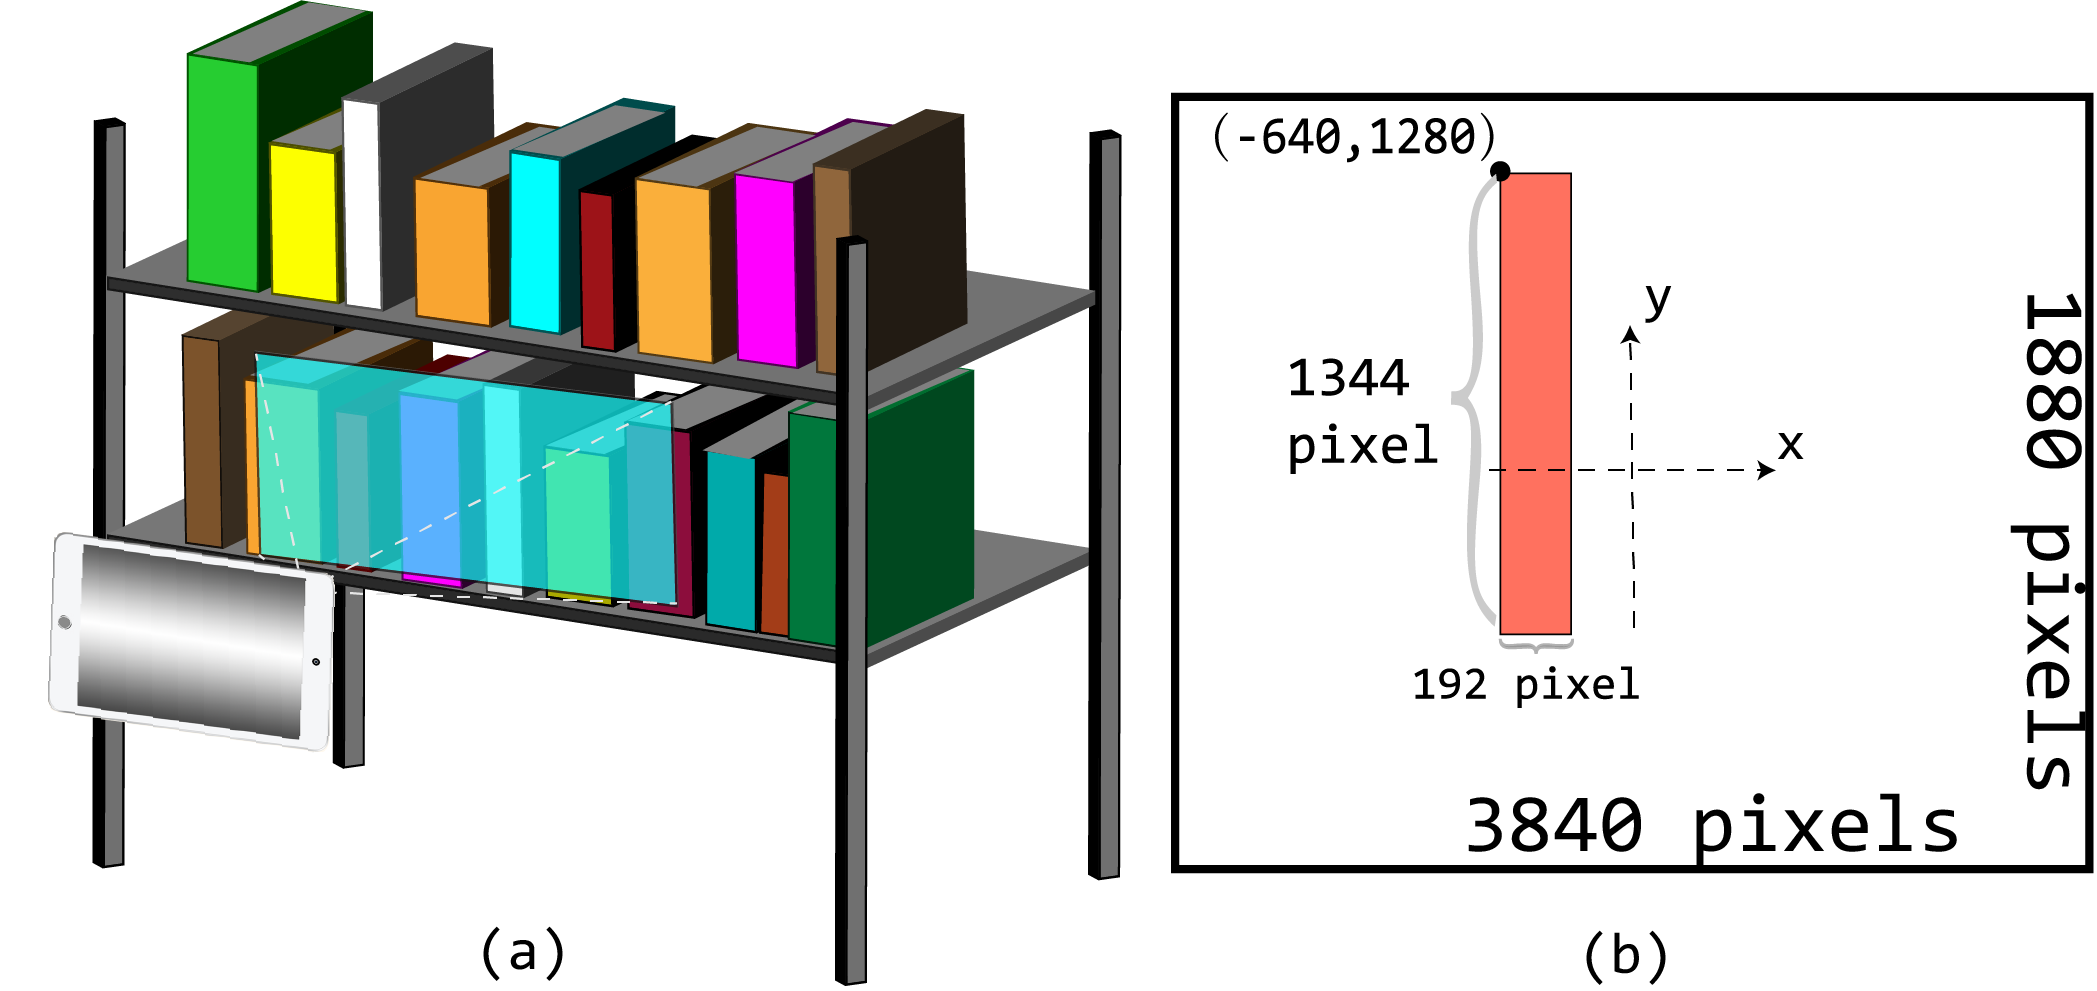
\includegraphics[width=\linewidth]{images/implementation_front.eps}
    \caption{
        (a) shows a mobile device is scanning the bookshelves.
        (b) is the top view of (a) showing the horizontal view angle $\alpha$,
        where $d$ is the distance between the mobile device and the target books estimated by \textit{ARLayout},
        and $x$ is the number of pixels horizontally.
        (c) shows a segmented book sample with the extracted position and size. %3840*1880
        % The coordinates of the top left corner of the book is (-640, 1280).
        (d) there are five blocks with recognized coffee names on a coffee menu.
    }
    \label{fig:implementation_front}
\end{figure}




%\subsection{Implementation}
%
%\textit{ARLayout} is based on C/S architecture
%that allows users to take photos/record videos in a cluttered environment
%using a mobile device such as iPad or other tablets.
%% The remote server processes the images in real-time, calculates the corresponding data feedback, and displays them by ARLayout.
%We tried \textit{ARLayout} in library, coffee shop, and cosmetics shop,
%three usage scenarios, where the objects will be
%re-grouped and re-ranked in AR space, and generate various augmented visual presentations.


\subsection{Database}

We create a large database on the server for
three application scenarios to serve these scenarios that
require real-time information feedback~\cite{Mcauley2015, He2016}.
% Some of this data is in the scenario itself, such as the title of the book, the name of the coffee, the price, and some of it is not in the scenario, but is related to the objects in the scenario, such as the book’s evaluation, the composition of the coffee.
Considering the additional information, the tool can better achieve design goal G4,
providing visual presentations or personalized recommendations by accessing the database in realtime.

% \textbf{Global Book Database}
% A database of more than 2 million books is created on the server, making it easy to quickly find the ISBN, title, author, author introduction, abstract, publisher, cover image, pages, prices, tags, ratings, reviews, etc.
% The dataset comes from jmcauley.ucsd.edu/data/Amazon/.

% The dataset comes from jmcauley.ucsd.edu/data/Amazon/, containing product reviews and metadata from Amazon, including 143.7 million reviews spanning May 1996 - July 2014. It includes reviews (ratings, text, helpfulness votes), product metadata (descriptions, category information, price, brand, and image features), and links (also viewed/also bought graphs).

% This means that we are only building a global database of books, but our application scenario is not limited to this. In similar application scenario, \textit{ARLayout} can also provide other data support through pattern matching algorithm. In other words, an interface for fast data import can be implemented in future work to meet the data service requirements of more scenarios. We will continue this topic in the Discussion section.

% \textbf{Coffee/Cosmetics Database}
% These two databases are created by the Web crawler, which crawled collection from well-known coffee, cosmetics brand website.
% For example, coffee data comes from Starbucks, including the coffee’s name, description, ingredients list, preview image, process introduction, while eyeshadow data mainly comes from Dior, including eyeshadow color, eye shape, location, use steps, tips, recommendations.

\subsection{Optical Character Recognition}


In the actual applications,
we found that the traditional OCR methods are not available for some complex scenarios,
e.g. slanted texts (\autoref{fig:implementation_ocr} (a)), %artistic fonts (\autoref{fig:implementation_ocr} (e)),
different text alignments in different languages (\autoref{fig:implementation_ocr} (c) and (d)).
The problems are that the English book texts (\autoref{fig:implementation_ocr} (c)) are often aligned in a vertical direction,
while the Chinese book texts (\autoref{fig:implementation_ocr} (d)) are often aligned in a horizontal direction.

In our experiments,
we improve the traditional OCR method, following a language adaptive design~\cite{Ling2018},
to achieve a large amount of the text characters over massive targets in reality.
In the approach, the texts of a book can be calibrated first if they are slanted,
and the language of a book will be identified first then the corresponding OCR
directions will be estimated,
which make the OCR recognition much more robust and scalable in the applications in reality.

%\textbf{Augmented OCR Network for Specific Scenarios}.
%Augmented template recognition works well when the texts are aligned well,
%e.g. the menu in a coffee shop.
%In the process of text recognition,
%the recognition template and classifier can be created according to different scenarios adaptively,
%which can automatically classify any regular format
%and output the recognition result in a structured way.
%In this section, there are two regions need to be settled.
%
%Reference region: the region pixels with fixed positions and contents
%in different pictures was chosen as anchor points of the picture,
%which can be used for template matching and rectification,
%as shown in~\autoref{fig:implementation_ocr} (f).
%Identification region: as shown in~\autoref{fig:implementation_ocr} (g),
%a field in a picture that needs to be identified
%was named to form a ``Key: Value'' relationship for ``Field name:
%Identification area content'',
%used to structurally identify the text contents.
%%of the same position of the same layout picture in real scenario.


\subsection{Image Segmentation and Labelling}

AR can effectively help users to migrate augmented information scenario
to real-world scenarios for observation.
Therefore, we use the method of image segmentation,
to help us segment and label the components from the image,
and then visualize the individual components in AR devices.
% In the actual implementation process, we sequential used the following methods to implement this function.

% \begin{figure}[htp]
%     \centering
%     \includegraphics[width=\linewidth]{images/BFS.eps}
%     \caption{
%         % (a) and (b) illustrate the process of BFS. In this image, each time the BFS cuts out the spine of a book.
%         (a) is the original photograph.
%         (b) is a single BFS expansion based on the pixel RGB values.
%         % (c) , (d) and (e) present scenarios that will have an negative impact on the effect.
%         (c) has several books of similar color, if they are adjacent, and the gap is very small, it may be considered as the same book.
%         (d) has a line between light and shadow in a shot, which can cause a book to be cut in half in poor lighting conditions.
%         (e) has a book with a color gap in its spine, and in real scenario it is possible that only the white parts are cut out.
%     }
%     \label{fig:BFS}
% \end{figure}

% \textbf{Breadth First Search}
% The algorithm was originally used for spine recognition in library/bookstore scenario. It is based on a basic assumption: the pixels at the spine of the book are basically continuous in RGB value. Therefore, on the basis of OCR, we approximate extend each text area with BFS algorithm until the pixel color transition too large, as shown in~\autoref{fig:BFS} (a) and (b). To show this process more clearly here, we have high-pixelated an area of the image. In real scenario, pixels extend by a much smaller step size (about 20 pixels per step, or 1/10 the size of the image). In the image, the green bolded edge points represent the current starting point, and the green unbolded edge points represent the feasible points that asingle BFS extension will reach. And the red points, represents the expanded RGB changes too large point. After a single BFS, all green points with unbolded edges will serve as starting points for the next round of BFS, continuing to expand the spine, while the red points will be discarded. At the end of algorithm, all the padding is the spine of a book.
% But this algorithm only based on RGB value, thus it shows high constraints in the actual use on the scenario, including lighting, spine design, etc. As shown in~\autoref{fig:BFS} (c) , (d) and (e). In addition, the assumption itself has a strong limitation: many objects do not have regular color separation. This means that the same algorithm is difficult to apply to other scenarios. Therefore, in the final version, we adopted the method of automatic segmentation of neural network to meet the needs of more scenarios.

\textbf{Convolutional Neural Network}.
To get a better result for various scenarios in real applications~\cite{Zhu2020},
we plan to use a convolutional neural network (CNN)-based approach
to do image segmentation and labelling.
We adopt an CNN-based open-source platform named PaddleSeg~\cite{Liu2019,Liu2021a}
to do image segmentation and labelling,
which just requires to manually annotate labels for a small amount of
samples for training (less than 100 for each usage scenario in this paper).
PaddleSeg is one of the state-of-the-art deep learning models for semantic image segmentation,
where the goal is to assign semantic labels (e.g., person, dog, cat and so on)
to every pixel in the input image.
In PaddleSeg, DeepLab~\cite{Chen2018} is one of its key modules.
Therefore, we take DeepLab as an example,
illustrating how PaddleSeg is integrated into \textit{ARLayout},
as shown in~\autoref{fig:implementation_network_deeplab}.
The encoder module encodes multi-scale contextual information by
applying atrous convolution at multiple scales, while the simple yet effective decoder
module refines the segmentation results along object boundaries.

%The panoramic pictures we captured or the real-time video we recorded
%are input into one of the three CNN networks (the top left of \autoref{fig:implementation_network}),
%while the labelled samples are input into the second CNN network (the top right of \autoref{fig:implementation_network}).
%Finally, the


\subsection{Coordinates Consistency between Virtuality and Reality}

To guarantee that the positions of the targets in AR space are consistent with their real-world positions,
we designed the coordinate transformation algorithm.
% This guarantees the virtual-world positions of targets consistent with their real-world position.
On the client-side, pictures taken by users are sent back to
the server for recognition.
The server sends back JSON data indicating the 2-D coordinates of targets in each picture.
If given an image with resolution of 3840*1880 as shown in~\autoref{fig:implementation_front} (c),
a red book is recognized at (-640,1280) with width 192 pixels and height 1344 pixels.
Whenever a picture is taken, we use ARKit to detect a possible virtual plane
in front of the camera, get the current transformation matrix $M_{plane}$,
and then compute the distance $d$ between the virtual plane and the
camera with LiDAR Scanner~\cite{ARKit}.



\subsection{Small Multiples and Virtual Models}

Regarding the visualizations for augmented information,
the related data will be sent to the server and the client will
receive the processed data from the server.
We design some visual presentation components like bar charts, line charts,
word cloud and the ingredients graphs, etc.,
which can be selected and composed for different usage scenarios.

We also create a virtual translucent screen in the AR environment to
show those augmented information.
Besides, in the eyeshadow scenario, we create a virtual head model,
stylize the model's eyes with the selected eyeshadow color
to show the 3-D preview presentations for users to help users
get a better fitting.


\begin{figure*}[htb]
%\setlength{\abovecaptionskip}{0.05cm}
%\setlength{\belowcaptionskip}{-0.4cm}
    \centering
    \includegraphics[width=\linewidth]{images/casestudy_book.eps}
    \caption{
        The user builds re-layouts and find books in a library.
        (a): The user scans the original bookshelves, 778 books recognized.
        (b): \textit{ARLayout} visualize the remaining books after fuzzy searching ``econimic''.
        (c): The user chooses to re-group by publisher, and searches ``Chicago''.
        Books from ``University of Chicago Press'' and other presses are placed on different layers.
        The user browses those books with fisheye effect.
        % The book in the middle of the screen will have its details (rating, author, publisher, price and Revewer's words) shown upon it.
        (d): The user searches ``social'' in books' names, several books are highlighted in red.
        (e): The user re-ranks those books by ratings. Books sorted
        in descending order are placed from the left to the right.
        (f): The user selects several candidate books, they are moved to a layer below.
        (g): \textit{ARLayout} shows books' word clouds.
        (h): The user compares books' ratings and prices via bar chart.
        (i): The user restores books to their original layout,
        and searches a book's name. The target book is highlighted in red.
        (j): The user finds and picks the target book according to its loation on the screen.
    }
    \label{fig:casestudy_book}
\end{figure*}

\begin{figure*}[htp]
%\setlength{\abovecaptionskip}{0.05cm}
%\setlength{\belowcaptionskip}{-0.4cm}
    \centering
    \includegraphics[width=\linewidth]{images/casestudy_coffee.eps}
    \caption{
        The user buinds re-layouts for a coffee menu.
        (a): The user scans the coffee menu%, 40 kinds of coffees are recognized.
        (b): The user search ``espresso''. Three related coffees are highlighted.% in red.
        (c): The user browses the menu with fisheye. The focused coffee will be magnified,
        with its summary shown besides it.
        (d): The user re-groupps all the drinks by sugar. %Four groups from ``Sugar Free'' to ``Sweet'' are shown.
        (e): The user selects four candidate coffees. They are moved to the right side of the menu% waiting to be compared.
        (f): The user compares candidate coffees by their ingredients graphs in small multiples.
        %in which different components and their amounts are clearly shown.
        (g): The user re-groupps drinks by fat. %Three groups with different fat contents are shown.
        (h): The user re-ranks drinks by calories. Drinks with more calories are moved to the left side.
 %while drinks with less calories are moved to the right.
        (i): The user compares the word cloud of the candidate coffees.
        (j): The user browses drinks on the right side of the menu to choose one with less calories.
    }
    \label{fig:casestudy_coffee}
\end{figure*}



\begin{figure}[htp]
    \centering
    \includegraphics[width=\linewidth]{images/casestudy_coffee_poster.eps}
    \caption{
        (a): The orignial poster hanging on the wall outside a coffee shop.
        (b): The user browses coffees' details with fisheye effect.
        (c): The user re-groups drinks by fat content intervals.
        (d): The user re-ranks drinks by calorie content.
    }
    \label{fig:casestudy_coffee_poster}
\end{figure}


\begin{figure*}[htb]
%\setlength{\abovecaptionskip}{0.05cm}
%\setlength{\belowcaptionskip}{-0.4cm}
    \centering
    \includegraphics[width=\linewidth]{images/casestudy_eye.eps}
    \caption{
        The user builds re-layouts for eyeshadows.
        (a): The user scans the various eyeshadows displayed on a cosmetics shop's desk.
        (b): The user re-groupps those eyeshadows by eyetypes, and views certain eyeshadow's
        details as well as a graph showing places to apply it on.
        (c): The user views the candidate eyeshadow's 3-D virtual makeup try-on.
        (d): The user re-groupps eyeshadows by high-rated scheme. Different schemes have features like ``Deep Blue'' or ``Soft Smokey''.
        (e): The user searches ``Scheme 13'' in their original layout, eyeshaodws contained in this scheme are highlighted.
    }
    \label{fig:casestudy_eye}
\end{figure*}



%As shown in in~\autoref{fig:implementation_front} (b), let $\alpha$ be the horizontal visual angle of the camera,
%$x$ be the number of horizontal pixels. Then the actual length
%of each pixel is calculated by:
%$$ l = \frac{2*d*\tan\frac{\alpha}{2}}{x} $$

%As shown in~\autoref{fig:implementation_front} (a), if a mobile device with visual angles 61\degree
% horizontally and 48\degree  vertically takes a picture of a bookshelf
%at the distance of 0.5m, it can be calculated that the red book in~\autoref{fig:implementation_front}(c) is 3cm thick and 21cm high,
%with its top left corner 0.1m left and 0.2m above the central of the plane.
%We multiply the plane's matrix with its corresponding translation to get the book's translation,
%and create a book model that's 3cm thick, 21cm high and 15cm long (we assume all books' length are $0.7*height$).


%The above coordinate transformation process is applied in the library/bookstore scenario and the eyeshadow scenario.
%While scanning a coffee menu, we don't record the plane matrix or the distance $d$,
%Instead, we use ARKit to recognize certain coffee menus dynamically.
%If ARKit recognizes a coffee menu that's same as the menu cropped from the server,
%we record and update the coffee menu's transformation matrix by each frame,
%attach an empty menu above the original menu,
%and generate coffee names in 3-D fonts with fixed sizes (a 7cm-high font for a poster,
%and a 1.5cm-high font for a smaller menu).
%Coffee names are placed in 5 groups that's similar to the original layout, as shown in~\autoref{fig:implementation_front} (d).
%In this way, as ARKit continuously updates the transformation of the recognized menu,
%the attached menu follows the real menu dynamically
%even the user moves the real menu.


%\subsection{Visual Presentations}
%
%We design some highlight \textit{ARLayout} d
%we use AR-based fisheye deformation to highlight
%the search results by flashing, transparency or AR-based fisheye deformation
%in the AR environment to guide them where to find the targets in the reality world.
%
%we use highlight effects will be applied to the searching results, i.e.,
%be magnified by 2 times and flash in red.
%This helps users locate their desired targets.
%
%When the user browses targets, fisheye highlight will be applied to those focused targets.
%The fisheye effect scaled targets close to the center of the screen.
%We project those recognized targets from their 3-D coordinates to 2-D screen pixel coordinates,
%calculate their distance $d$ to the screen center.
%If $d$ is less than a threshold $d_{min}$, we calculate their magnification ratio $r$ as follows:
%$r =  max(2,\frac{d+a}{d}) $ ($a$'s value changes according to different devices, in a 11-inch iPad-Pro, 30 is recommended).
%As a result, targets closer to the screen center is scaled to an appropriate degree.
%
%The target closest to the screen center will have its summary shown up in a panel beside it.
%The panel will have its position updated every frame based on the target's projected 2-D screen pixel coordinates,
%so that the summary panel will follows the focused target when it moves on the screen.

%\subsection{Searching, Re-grouping and Re-ranking}
%
%When the user searches for targets' certain attribute,
%we traverse the scanned targets' attributes, and generate a list of targets
%with attributes containing the input text.
%
%In terms of re-grouping, targets will be arranged in a new layout according to their groups.
%In the library/bookstore scenario, we create virtual bookshelves in front of the user,
%and place groups of books on different layers of the bookshelves.
%The process is as follows:
%first, we multiply the current transformation matrix of the device with a forward translation
%to get the transformation of the bookshelves.
%Then we move different groups of books onto the shelves, and show their group names with a 0.1m-height 3-D font.
%% The book models' translation is similar to the bookshelves translation, but with different $x$, $y$ and $z$ so that they
%% move to the corresponding layers of the bookshelves.
%To reduce visual complexity, we place a semitransparent white plane at the back of the bookshelves
%so that the real books captured by the camera are dimmed.
%In the coffee shop scenario, different groups of coffees will be placed in different blocks.
%If one group has too many coffees that can't be all shown in one block, those exceeded will be hidden.
%The user can touch and drag the block to roll up the coffee list and show the hidden ones.
%In eyeshadow scenario, eyeshadows in a same group is re-layouted in rows.
%A semitransparent white plane is also placed behind them to avoid visual conflicts.


%\textit{ARLayout} can also re-rank targets based on different dimensions.
%We generate a new list containing targets' indexes sorted by certain dimension.
%In the library/bookstore scenario, sorted books will be lined up on the bookshelves.
%In the coffee shop scenario, sorted coffees will have their names shown in the designed blocks.
%Each block shows a group whose attributes falls into certain interval.
%For example, when sorted by calories, ``Block one'' lists the highest ten coffees that contains
%the most calories ($380 cal - 240 cal$).

% If the user selects several targets, they will move to the alternative area (Figure A).
% In the library scenario, the user can compare ratings and prices of the selected books by







\section{Usage Scenarios}

To illustrate how \textit{ARLayout} searches, re-groups and re-ranks massive physical targets
in AR environments,
we describe three usage scenarios where users use \textit{ARLayout} to
search and filter targets, obtain their information, and locate
ideal ones among massive targets,
i.e., the usage scenarios in a library/bookstore, a coffee shop and an eyeshadow fitting.

\subsection{Library/Bookstore Scenario}

Suppose Zelda is a student major in economy.
She wants to buy some economic books to broaden her horizons.
She prefers books from the ``University of Chicago Press'',
which is recognized as having been publishing high-quality books.
She comes to the social science area in a library/bookstore,
facing a large row of bookshelves with around 1000 books.
Instead of looking for books in the bookstore's searching system (which is often just
open for bookstore clerks),
by which she may have dizzy and tedious choosing experience.

(1) \textbf{Fuzzy searching/filtering}: she decides to quickly scan the whole bookshelves by the panoramic camera by \textit{ARLayout}.
Soon 778 books are recognized in total.
She then filters unrelated books by saying ``economic''.
\textit{ARLayout} deals with the voice input, and filters those books by fuzzy search.
% fisheye
Seeing that only 118 economic books remains, Zelda chooses to visualize those books
in the AR space and browses them as shown in~\autoref{fig:casestudy_book} (b).
She finds that only one book nearby is from ``University of Chicago Press'',
then she want to find more books on ``economic' and published by ``University of Chicago Press''.

% re-groupp
(2) \textbf{Re-grouping}: she re-group those 118 books by publisher and searches by saying ``Chicago''
or inputting by the virtual keyboard of her mobile phone.
This time, seven books from the ``University of Chicago Press'' are highlighted and
placed on a bookshelf in front of her with fisheye effect (\autoref{fig:casestudy_book} (c)).
Books from other presses are also grouped and placed on the other layers of the
shelf (\autoref{fig:casestudy_book} (d)), so she choose a book from them.

% search
(3) \textbf{Fuzzy re-searching}: she wants to search all books with fuzzy keyword ``social'' ,
there are 21 books highlighted in red (\autoref{fig:casestudy_book} (d)).
She uses fisheye effect to view each book's details like author and reviewers' words (\autoref{fig:casestudy_book} (c)).
But she finds these social books are not highly rated or the authors are not in her favorite author list,
So she changes idea: she re-ranks those books by ratings or further filter them by author names.

% re-rank
(4) \textbf{Re-ranking}: she sort all of the books which are placed
from left to right on the same layer of the shelf by descending order (\autoref{fig:casestudy_book} (e)).
Then she selects four books that seems suitable,
those selected books are moved to a lower layer of the
virtual bookshelf where are designed to place the candidate books (\autoref{fig:casestudy_book} (f)),
just like a shopping cart.

% word cloud
(5) \textbf{Comparing by word cloud visualizations in small multiples}:
she views and compares the word cloud of each book's keywords.
Among those four books, one book has keywords ``story'' and ``understand'', other books' keywords are
``city'', ``environmentalist'' and ``empire'' (\autoref{fig:casestudy_book} (g)).
Zelda is interested in the ``story'' one and the ``empire'' one, but she's also concerned with the prices
if she is going to buy in a bookstore.


(6) \textbf{Comparing with kinds of diagrams in small multiples}:
so she compares these books' ratings and prices together
in the bar chart (\autoref{fig:casestudy_book} (h)).
She finds that the ``story'' (the first) rated as high as
the ``empire'' one (the fourth), but is a little cheaper than the ``empire'' one.
So she choose the ``story'' one and restores those books to their original layout.

(7) \textbf{Title Precise Searching}: finally, she voice input the title ``human resources management''.
The book is magnified and highlighted on the left upper side (\autoref{fig:casestudy_book} (i)) by flashing.
She walks by and locates the book in the reality space according to
its position shown in the screen (\autoref{fig:casestudy_book} (j)).




% \begin{figure}[htp]
%     \centering
%     \includegraphics[width=\linewidth]{images/books.eps}
%     \caption{
%      coffee menu.
%     }
%     \label{fig:casestudy}
% \end{figure}

% Another day, Zelda wonders in a book shop looking for interesting books to read.
% She walks to the history area and plans to choose some books about economics.
% She scans those shelves and \textit{ARLayout} recognize about 1500+ books. She then input
% "economic" by voice. After fuzzy search and filtering, 118 books remains.
% % She visualizes those books, and views their details by fisheye effect.
% However, she's not familiar with economic books' publishers and authors,
% so she re-ranks those books by ratings. A virtual shelf shows up, with books sorted by
% descending order placed from left to right.
% Then she browses books with fisheye effect from left to right,
% chooses 4 books with appealing titles.
% She compares the word cloud of those books and find that they all suit her taste.
% She then compares the ratings and prices by charts, chooses the book "" with a relatively high price–performance ratio.
% Then, similar to finding the algorithm book previously, she restores virtual books, searches the title,
% and successfully finds the ideal book in the real space.

% \begin{figure}[htp]
%     \centering
%     \includegraphics[width=\linewidth]{images/Cafe.eps}
%     \caption{
%         virtual coffee menu.
%     }
%     \label{fig:casestudy}
% \end{figure}

\subsection{Coffee Shop Scenario}

A new coffee shop opens in Zelda's campus.
she don't know much about coffee,
but is willing to try some in the new coffee shop.
She walks in the coffee shop, takes a picture of the coffee menu by \textit{ARLayout}.
Soon it recognizes 40 different drinks, and creates a menu upon the original one.
% She browses the menu using fisheye effects,

She remembers that she once ordered a cup of espresso,
which she thinks is rather bitter, so she wants to see the ingredients.
% To compare espresso with other coffees,
So she firstly voice inputs ``Espresso'' and finds that
it's highlighted in the ``Hot Coffees'' group(\autoref{fig:casestudy_coffee} (b)).
She views the details of Espresso, learns that it's surely bitter,
as no sugar is added in it (\autoref{fig:casestudy_coffee} (c)).

She then re-groups those drinks according to milk or sugar (\autoref{fig:casestudy_coffee} (d-e)).
She browses and selects some drinks with high ratings in the ``medium sweet''
and ``sweet'' group, as shown in~\autoref{fig:casestudy_coffee} (f).
Then she compares those drinks' ingredients in small multiples,
and finds that Cappuccino has a balance between sugar, milk and caffine,
which may suit to her taste, as shown in~\autoref{fig:casestudy_coffee} (g).
However, her fitness coach's advice cross her mind that she needs to limit the calorie intake to 1300 calories everyday,
while the coffee summary shows that Cappuccino has 140 calories per cup.
So she re-ranks all the drinks by calorie content.
This time, coffees are sorted from left to right by calorie,
as shown in~\autoref{fig:casestudy_coffee} (h).
She begins browsing on the right side, where coffees with relatively low calorie are located.
She find some of coffees that she haven’t drunk.
To have a quick grasp of them, she views their word cloud (\autoref{fig:casestudy_coffee} (i)).
She learns that Blonde Roast is regarded to be ``mellow'' in the word cloud,
Iced Coffee is ``rich'',
and Caffee Americano has keyword ``espresso'', which may be too bitter for her.
% She again searches the Blonde Roast, find that it locates to the right of
% the menu where coffees with relatively low calorie content are located(shown in~\autoref{fig:casestudy_coffee} (e)).
She browses Blonde Roast's summary, which confirms that it only contains five calories per cup (\autoref{fig:casestudy_coffee} (j)).
Finally, she chooses Blonde Roast and enjoys its ``soft and mellow flavor'' described in the summary.

In addition, \textit{ARLayout} can also handle larger menus like the poster hanging on the wall
outside the coffee shop, as shown in~\autoref{fig:casestudy_coffee_poster} (a).
The user can view details var fisheye, re-group, re-rank, select and compare drinks on the poster, 
which is similar to the smaller menu, as shown in~\autoref{fig:casestudy_coffee_poster} (b-d).


% Since Zelda has an enjoyable experience learning and choosing drinks in the coffee shop,
% several days later, she visits the coffee shop again.
% % , planning to explore and try something different.
% This time, she plans to explore and try something different.
% "Maybe coffees with no milk", she thinks.
% She scans the menu and starts browsing in virtual space.
% Firstly, she re-groupps the drinks according to milk content.
% In the "<=5\%" group, she selects some coffee and drinks.
% To have a quick grasp of these drinks, she views their word cloud(shown in~\autoref{fig:casestudy} (j)).
% She learns that the Iced Coffee in this coffee shop is regarded as "rich",
% Blonde Roast is "mellow",
% and Caffee Americano has keyword "espresso", which may be too bitter for her.
% Before deciding between Blonde Roast and Iced Coffee,
% she remembers her fitness coach's advice of limiting the calorie intake everyday.
% So she re-ranks all the drinks by calorie content.
% She then searches these two coffees,
% finds that Iced Coffee locates at the left side of the menu where drinks contains more calories,
% while Blonde Roast locates at the right side, indicating its relatively low calorie content(shown in~\autoref{fig:casestudy} (k)).
% The fisheye effect confirms that Blonde Roast only contains 5 calories per cup(shown in~\autoref{fig:casestudy} (l)).
% Finally, she chooses Blonde Roast and enjoys its soft and mellow flavor.


\subsection{Eyeshadow Scenario}

One day Zelda is shopping in a cosmetics shop.
She is not good at making up, especially eyeshadow,
because different eyeshadows may have unique effects,
and sometimes several eyeshadows may be applied to different places
to form a colour combination.
So she uses \textit{ARLayout} and scans those eyeshadows displayed on the desk, as shown in~\autoref{fig:casestudy_eye} (a).
Soon 15 different eyeshadows with 96 different colors (or textures) are recognized.
She then re-groups them by eyetypes, and use fisheye effect to view the details of the ``protruding eye'' group,
as shown in~\autoref{fig:casestudy_eye} (b).
% Those slightly different eyeshadows in this color group may have their unique effects.
A graph pops up on the side of the selected eyeshadow, showing the ideal position for users to apply it on.
Zelda chooses a kind of golden brown eyeshadow,
and previews its 3-D effect on a virtual model, as shown in~\autoref{fig:casestudy_eye} (c).
Zelda still finds it hard to choose several eyeshadows that matches each other,
so she re-groups them by high rated schemes, this time,
three recommended color schemes are lined up in front of her, as shown in~\autoref{fig:casestudy_eye} (d).
Zelda views the details about each eyeshadow's effects and features,
learns that eyeshadows in ``Scheme 13'' is suitable for simple day look.
So she restores those colors to their original layout and search for ``Scheme 13'' by voice.
Those eyeshadows in ``Scheme 13'' are flashing in red, as shown in~\autoref{fig:casestudy_eye} (e).
As a result, she chooses an eyeshadow palette that contains
some colors in ``Scheme 13''.
% Details about each eyeshadow's effects and features are shown on the UI.

% There's also details  about its features and style.


\section{Discussion and Future Work}
\label{sec:discussion}

We discuss the limitations and some potential extension work of this paper
in this section.

%\subsection{Limitations}

We design a personal visualization tool named \textit{ARLayout}
for non-experts without programming knowledge
to build AR-based visual re-layouts towards massive physical targets.
We summarize the salabilities and some limitations of \textit{ARLayout} as follows:

\textbf{The scalability of application scenarios}. Except the usage scenarios presented in the paper,
the current version of \textit{ARLayout} supports various application scenarios where:
(1) the targets with textual information such as menus of coffee, drinks, foods, etc.,
goods in supermarkets with name-price labels,
or even a large number of cars in a parking lot (license plates), etc.
(2) the targets with colors such as eyeshadow,
colored balls or balloons in a large amusement park,
the colored goods in supermarkets, etc.
(3) the targets with 2-D shapes and some simple 3-D shapes like tables, chairs, windows, etc., 
however, it is not applicable for complex 3-D shapes due to
the limitations of image labelling algorithms towards various 3-D objects. 

\textbf{Rendering limitation of AR devices}.
We used the latest 11-inch 2021 iPad-Pro with A12Z processor,
which is one of the top end configuration for the nowadays iPad with ARKit.
The framework could visualize the AR targets (actually are virtual targets)
in AR environment well when the number is below 200.
However, as the target number increases, the frame rate drops.
%This situation appears more in the library/bookstore scenario, where the number of books often exceeds 1000.
Though several experiments, we found that the frame rate stabilizes at 60 per second
when the number of targets (e.g., books in the library scenario) is below 200, and decreases to 30 frames per second
if it exceeds 230. Furthermore, if AR books' number increases to 320, the frame rate
will drop significantly to below 15.

Nevertheless, this limitation (low FPS when the target number grows larger than 320)
mainly restricted by the current mobile device would \textbf{not appear} if users
follow a rountine task workflow, i.e.,
searching the targets first to narrow down the number of candidates to 320 or less.
The more unrelated targets are filtered out, the more efficient and the more effective
the users can fulfill their tasks.
For example, users can search books with a fuzzy keyword ``data structure''
to decrease the data space significantly,
and then the subsequent tasks including re-grouping, re-ranking or further searching
will be visualized fluently enough in AR environment.
The major issue of this limitation is that the AR device can not show
too many AR objects (e.g., larger than 320).

It is worth noting that the image segmentation and labelling components of \textit{ARLayout}
are \textbf{scalable} and \textbf{not limited} by the target number,
because the convolutional neural network and the OCR algorithm are run on the server
which can even handle thousands of books in the library usage scenario in our experiments.
More importantly, unlike the mobile device, the computation resources of the server are
\textbf{scalable enough} and which could be upgraded easily.
As a result, while \textit{ARLayout} recognizes almost all the books scanned by the user,
we recommend the user to first filter out unrelated books by fuzzy searching before actually
visualizing those books in the AR space in order to narrow down the data space.


\textbf{Image resolution limitation}. \textit{ARLayout} recognizes objects by images taken from the mobile devices.
Ideally, the user only need to take one panoramic picture that contains all the target objects.
However, targets' details may not be recognized if they are too small in the picture,
that is the user is stand too far away from the massive targets.
For example, in the library/bookstore scenario, instead of scanning all layers of the bookshelves,
the user may walk closer to the bookshelves and scan one layer at one time by panoramic stitching
due to lack of light or limited imaging quality.



%\subsection{Future Work}
We plan to optimize the following aspects of \textit{ARLayout} in future work:

\textbf{More complex application scenarios support.} Currently \textit{ARLayout} is capable of recognizing books, coffee names,
drinking menu, food menu, or eyeshadows.
In the future, we plan to expand its usage scenarios to other similar ones like choosing cups, fruits or flowers, etc.
Because targets with text on it, or in different colors and shapes can be well recognized by trained neural networks.
During targets recognition, targets' additional information is acquired from the database,
so an interface for fast data import can be implemented
in future work to meet the data requirements of more scenarios.

%\textbf{Real-time position sync between virtuality and reality.}
%The current version of \textit{ARLayout} can
%accurately creates virtual targets in the AR environment
%whose position is consistent with the real world targets.
%% and is able to accept simple changes in the scenario,
%such as following the targets shaking,
%but there is still a long way to go with the dynamic scenarios.
%For example, it is extremely difficult for the current \textit{ARLayout} to use AR
%to dynamically capture the changes of players in a football match.
%But the basic algorithm of AR,
%such as plane tracking and 3-D targets recognition,
%have reached quite performance requirements.
%Therefore, the difficulty of moving \textit{ARLayout} from static scenario to dynamic scenario
%depends on the real-time data processing.

\textbf{Detailed Texture Recognition in AR}. Some of user study participants
consider it could be better to use the same texture to show the AR effects,
especially in the eyeshadow scenario.
At present, the preview effect of eyeshadow only stays at the transfer of RGB value.
Further study with more focus on detailed texture recognition is therefore suggested,
e.g., the eyeshadow texture on glossiness or oiliness, etc.
A Deep Texture Encoding Network (DeepTEN) with a novel Encoding Layer
integrated on top of convolutional layers offers possibilities
to solve this problem~\cite{Zhang2017}.
Besides, we are trying to use a better architecture,
such as abandoning the server if the mobile device is affordable
and building a lightweight neural network to move them to run on the mobile devices.



% \textbf{Interface for data import}
% During targets recognition, targets' additional information is aquired from the database.
% which means that in similar usage scenario,
% \textit{ARLayout} can also provide data support through pattern matching algorithm.
% In other words,
% an interface for fast data import can be implemented
% in future work to meet the data requirements of more scenarios.

%\textbf{Automatic scenario recognition}
%When using the current ARLayout,
%users need to classify the current scenario type,
%and then choose the corresponding recognition mode,
%which often leads to inconvenience in using.
%The complexity of the scenario requires
%\textit{ARLayout} to be designed with scenario understanding
%to avoid the difficulty of describing the current scenario type
%when users facing an unknown scenario.
%Recently, the research on computer vision on visualization
%has provided AI's scenario automatic recognition function,
%which make it possible for environment adaptive visualization~\cite{Andreu2011}.

% \textbf{Relatedwork Comparison}
% The most related work of \textit{ARLayout} are some authoring tools towards AR or VR visualizations.
% As shown in Table~\ref{tab:discussion_relatedwork_cmp},
% we compare them from eight aspects:
% highlight(fisheye), collabration, searching, re-grouping, re-ranking,
% massive targets, glyph vis, augmented infomation.
% We summarize them into six criterias:
% more intuitive interaction, personal or collaborated,
% layout changes or keep origin layout,
% a few targets or massive targets, whether glyph used,
% use the original information or add more information.

% \begin{table}[htp]
%     \centering
%     \includegraphics[width=\linewidth]{images/discussion_relatedwork_cmp.eps}
%     \caption{
%         Comparison to the most related recent work about authoring tools
%         towards AR or VR visualizations.
%     }
%     \label{tab:discussion_relatedwork_cmp}
% \end{table}

\section{Conclusion}

%In this work, we present \textit{ARLayout},
%an authoring tool designed for non-experts
%to build AR-based visual re-layouts over massive physical targets.
%The design and implementation of \textit{ARLayout} is based on the C/S architecture.
%OCR and image segmentation are used to process the text and image data in the scenario,
%and AR + VR (mainly AR) are used to display the data.
%We demonstrate the expressiveness, usability and usefulness of \textit{ARLayout}
%through three usage scenario examples and a user study.


In this paper, we present \textit{ARLayout}, a personal visualization tool designed
for non-experts to build AR-based visual re-layouts towards massive physical targets,
such as books in a library/bookstore, coffees in a coffee shop, eyeshadows in a shop, etc.
The real-time video are captured from the reality world by the camera of
mobile devices.
All the candidate targets can be segmented and labeled by
a convolutional neural network PaddleSeg~\cite{Liu2019,Liu2021a}.
The network just requires a small scale of labeled training
samples, i.e., less than 100 for each case in our experiments,
while the textual information is recognized by an OCR algorithm.

The visual re-layouts of the physical targets include (1) highlighting
the search results by AR-based fisheye deformation,
(2) re-grouping them according to their additional nominal,
ordinal or quantitative attributes,
and (3) re-ranking them according to their additional ordinal or quantitative attributes.
In the searching scenario, the fuzzy keywords are input by voice to narrow down the number of candidate targets,
and then the search results will be highlighted by flashing, transparency or AR-based fisheye deformation
in the AR environment to guide them where to find the targets in the reality world.
In the re-grouping task, candidate targets can be re-grouped in the AR environment
according to one or multiple of their nominal, ordinal or quantitative attributes.
In the re-ranking task, candidate targets can be sorted in the AR environment according to one of
their ordinal or quantitative attributes.
In the experiments, we demonstrate the usability, expressiveness and effectiveness
of \textit{ARLayout} by a user study and three case studies.

%%%--------------------------------------------------------------------------------%%%



%% if specified like this the section will be committed in review mode
\acknowledgments{
The authors wish to thank A, B, and C. This work was supported in part by
a grant from XYZ (\# 12345-67890).}

%\bibliographystyle{abbrv}
\bibliographystyle{abbrv-doi}
%\bibliographystyle{abbrv-doi-narrow}
%\bibliographystyle{abbrv-doi-hyperref}
%\bibliographystyle{abbrv-doi-hyperref-narrow}

\bibliography{arlayout}
\end{document}

